\documentclass[10pt,xcolor=pdflatex, table]{beamer}
\usepackage{newcent}
\usepackage[utf8]{inputenc}
\usepackage[czech]{babel}
\usepackage{hyperref}
\usepackage{textpos}
\usepackage{multicol}
\usepackage{tikz}
\usepackage{fancyvrb}
\usepackage{color}
\usepackage{subfig}
\usepackage{geometry}
\usepackage{graphicx}
\usepackage{pgf}
\usepackage{epstopdf}
\usepackage{todonotes}

\epstopdfDeclareGraphicsRule{.gif}{png}{.png}{convert gif:#1 png:\OutputFile}
\AppendGraphicsExtensions{.gif}
\usetheme{FIT}

\def\uv#1{\quotedblbase#1\textquotedblleft}%
\newcommand{\putat}[3]{\begin{picture}(0,0)(0,0)\put(#1,#2){#3}\end{picture}}

%%%%%%%%%%%%%%%%%%%%%%%%%%%%%%%%%%%%%%%%%%%%%%%%%%%%%%%%%%%%%%%%%%
\title[GJA 6]{Spring}

\author[]{Jaroslav Dytrych, David Koz\'ak}

\institute[]{Faculty of Information Technology
Brno University of Technology \\
Bo\v{z}et\v{e}chova 1/2. 612 66 Brno - Kr\'alovo Pole\\
dytrych@fit.vutbr.cz}

\date{7 November 2023}
%\date{\today}
%\date{} % bez data

%%%%%%%%%%%%%%%%%%%%%%%%%%%%%%%%%%%%%%%%%%%%%%%%%%%%%%%%%%%%%%%%%%

% TODO:
% * @Required is deprecated (SpringAnnotations example) https://docs.spring.io/spring-framework/docs/current/javadoc-api/org/springframework/beans/factory/annotation/Required.html
%

\begin{document}

\frame[plain]{\titlepage}

\bluepage{Spring}

\begin{frame}\frametitle{Contents}
  \begin{itemize}
    \item IoC (Inversion of Control)
    \item Spring Introduction
    \item Annotations
    \item Configuration
    \item Transactions
    \item \textbf{Events}
    \item \textbf{Aspects}
    \item \textbf{Spring Web MVC} (beans for Model, JSP for View and Spring for Controller)
    \item \textbf{Security}
    \item \textbf{Spring Boot}
  \end{itemize}
\end{frame}

\begin{frame}\frametitle{IoC (Inversion of Control)}
  \begin{itemize}
    \item Some parts of our code receives the flow of control from a~generic framework.
    \item Principle ``Don't call us, we'll call you.''
    \item Instances of classes are not created but they are provided externally. Class do not need to know about implementation of an interface.
    \item Mostly used techniques are:
      \begin{itemize}
        \item Constructor Injection -- constructor is able to receive needed objects,
        \item Setter Injection -- class have a setters for necessary objects,
        \item Interface Injection -- interface with setters for necessary objects is defined, class have to implement this interface.
      \end{itemize}
    \item Advantages:
      \begin{itemize}
        \item Less dependencies between particular classes.
        \item Explicitly specified dependencies.
        \item Less type casting.
        \item Better reusability of components.
      \end{itemize}
    \item Disadvantages:
      \begin{itemize}
        \item It is more complicated to understand the code.
      \end{itemize}
  \end{itemize}
\begin{tikzpicture}[remember picture,overlay]
    \node[xshift=-0.6cm,yshift=-1.3cm] at (current page.north east){%
    
\includegraphics[width=1cm]{img/pozor}};
\end{tikzpicture}
\end{frame}



\begin{frame}\frametitle{What is Spring}
	\begin{itemize}
		\item One of the most popular application development frameworks for enterprise Java.
		\item Spring makes JavaEE development easier.
		\item Benefits
          \begin{itemize}
        	\item Working with POJOs (no enterprise containers)
        	\item Modular framework
        	\item Can be combined with many other technologies
        	\item Framework for web with MVC
        	\item API for JDBC (Java Database Connectivity), Hibernate
        	\item IoC containers, dependency injection
        	\item Consistent transaction management
          \end{itemize}
	\end{itemize}
\end{frame}


\begin{frame}\frametitle{Dependency injection}
	\begin{itemize}
		\item Dependency injection is example of IoC.
		\item Makes writing of reusable and independent components possible.
          \begin{itemize}
        	\item Glues them together.
          \end{itemize}
		\item Dependency injection in Spring can happen in the way of passing parameters to the constructor or by post-construction using setter methods.
	\end{itemize}
\begin{tikzpicture}[remember picture,overlay]
    \node[xshift=-0.6cm,yshift=-1.3cm] at (current page.north east){%
    
\includegraphics[width=1cm]{img/pozor}};
\end{tikzpicture}
\end{frame}


\begin{frame}\frametitle{Aspect oriented programming (AOP)}
	\begin{itemize}
		\item Cross-cutting concerns are conceptually separate from the application's business logic.
		\item Examples
          \begin{itemize}
        	\item Logging
        	\item Transaction management
        	\item Security
        	\item Caching
          \end{itemize}
		\item Defining method interceptors and pointcuts
          \begin{itemize}
            \item Pointcuts for events
            \item Interceptors handles events
          \end{itemize}
	\end{itemize}
\begin{tikzpicture}[remember picture,overlay]
    \node[xshift=-0.6cm,yshift=-1.3cm] at (current page.north east){%
    
\includegraphics[width=1cm]{img/oko}};
\end{tikzpicture}
\end{frame}


\begin{frame}\frametitle{Spring architecture}
\begin{center}
  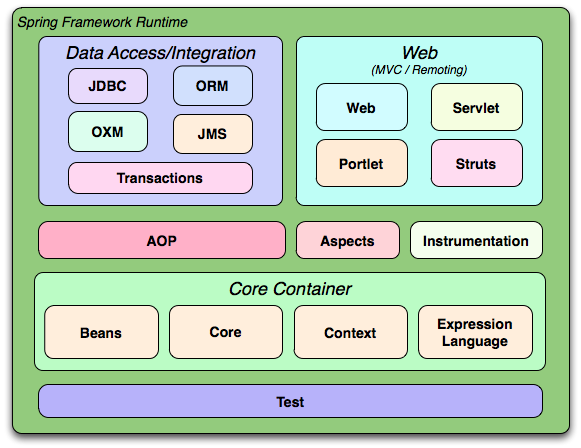
\includegraphics[scale=0.5]{img/obr1}
\end{center}
\begin{textblock}{15}(1.3,-0.3)
    {\footnotesize ORM -- Object/Relational Mapping, OXM -- Object/XML mapping}
\end{textblock}
\begin{textblock}{15}(1.3,-13.8)
    {\footnotesize Portlet -- more servlets on the one page (generating fragments)}
\end{textblock}
\end{frame}


\begin{frame}\frametitle{Core container}
	\begin{itemize}
		\item The Core module provides the fundamental parts of the framework, including the IoC and Dependency Injection features.
		\item The Bean module provides \texttt{BeanFactory} which is a~sophisticated implementation of the factory pattern.
		\item The Context module provides \texttt{ApplicationContext} interface, through which configured objects are accessible.
		\item The Expression Language module provides a powerful expression language for querying and manipulating an~object graph at runtime.
	\end{itemize}
\end{frame}


\begin{frame}\frametitle{Data access/integration}
	\begin{itemize}
		\item JDBC (Java Database Connectivity) abstraction layer.
		\item The ORM module provides integration layers for popular object-relational mapping APIs, including JPA (Java Persistence API), JDO (Java Data Objects), Hibernate, and~iBatis.
		\item The OXM module provides an abstraction layer that supports Object/XML mapping implementations for JAXB, Castor, XMLBeans, JiBX and XStream.
		\item The JMS module contains features for producing and consuming messages.
		\item The Transaction module supports programmatic and declarative transaction management for classes that implement special interfaces and for all your POJOs.
	\end{itemize}
\end{frame}


\begin{frame}\frametitle{Web}
	\begin{itemize}
		\item Web
          \begin{itemize}
            \item provides basic web-oriented integration features
        	\item Multipart fileupload
        	\item Initialization of IoC container
        	\item Servlet listeners, application context
          \end{itemize}
		\item Web-Servlet module
          \begin{itemize}
        	\item Model-View-Controller (MVC)
          \end{itemize}
		\item Web-Struts
          \begin{itemize}
        	\item Integration with Struts framework (MVC with strict rules)
        	\item deprecated as of Spring 3.0 -- use Struts 2.0 and its Spring integration or Spring MVC solution instead
          \end{itemize}
        \item Web-Portlet
          \begin{itemize}
        	\item MVC implementation to be used in portlet environment
        	\item Mirrors functionality of Servlet
          \end{itemize}
	\end{itemize}
\end{frame}


\begin{frame}\frametitle{Spring HelloWorld}
	\begin{itemize}
		\item Create POJO object.
		\item Create Bean configuration file.
		\item Get application context.\\
          \begin{itemize}
        	\item \texttt{ClassPathXmlApplicationContext("Beans.xml");}
          \end{itemize}
		\item Get POJO bean.
		\item Perform bean functionality.
	\end{itemize}
\begin{tikzpicture}[remember picture,overlay]
    \node[xshift=-0.6cm,yshift=-1.3cm] at (current page.north east){%
    
\includegraphics[width=1cm]{img/lupa}};
\end{tikzpicture}
\end{frame}


\begin{frame}[fragile]\frametitle{Spring HelloWorld}
\begin{Verbatim}[fontsize=\footnotesize, commandchars=\\\{\}]
\textcolor{purple}{\textbf{public class}} MainApp \{
    \textcolor{purple}{\textbf{public static void}} main(\textcolor{purple}{\textbf{String[]}} args) \{
        ApplicationContext context =
            \textcolor{purple}{\textbf{new}} ClassPathXmlApplicationContext(\textcolor{blue}{"Beans.xml"});
        HelloWorld obj =
            (HelloWorld) context.getBean(\textcolor{blue}{"helloWorld"});
        obj.getMessage();
    \}
\}

\textcolor{purple}{\textbf{public class}} HelloWorld \{
    \textcolor{purple}{\textbf{private String}} message;
    \textcolor{purple}{\textbf{public void}} setMessage(\textcolor{purple}{\textbf{String}} message)\{
        \textcolor{purple}{\textbf{this}}.message = message;
    \}
    \textcolor{purple}{\textbf{public void}} getMessage()\{
        System.out.println(\textcolor{blue}{"Your Message : "} + message);
    \}
\}

<bean id=\textcolor{blue}{"helloWorld"} class=\textcolor{blue}{"cz.vutbr.fit.HelloWorld"}>
    <property name=\textcolor{blue}{"message"} value=\textcolor{blue}{"Hello World!"}/>
</bean>
\end{Verbatim}
\begin{tikzpicture}[remember picture,overlay]
    \node[xshift=-0.6cm,yshift=-1.3cm] at (current page.north east){%
    
\includegraphics[width=1cm]{img/lupa}};
\end{tikzpicture}
\end{frame}


\begin{frame}\frametitle{Spring IoC containers}
\begin{center}
  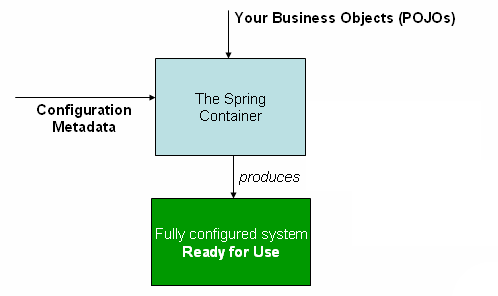
\includegraphics[scale=0.65]{img/obr2}
\end{center}
\begin{tikzpicture}[remember picture,overlay]
    \node[xshift=-0.6cm,yshift=-1.3cm] at (current page.north east){%
    
\includegraphics[width=0.8cm]{img/pozor}};
\end{tikzpicture}
\end{frame}


\begin{frame}[fragile]\frametitle{Spring IoC containers}
	\begin{itemize}
		\item BeanFactory container
          \begin{itemize}
        	\item Basic support for dependency injection.
            \item Class \texttt{XmlBeanFactory} (deprecated).
        	\item Various interfaces for backward compatibility.
          \end{itemize}
        \item ApplicationContext container
          \begin{itemize}
        	\item More enterprise-specific functionality.
        	\item Wire beans together.
        	\item Recommended over BeanFactory.
        	\item \texttt{FileSystemXmlApplicationContext} -- full path to XML
        	\item \texttt{ClassPathXmlApplicationContext} -- XML on ClassPath
        	\item \texttt{WebApplicationContext} -- for web applications (\texttt{WEB-INF})
          \end{itemize}
	\end{itemize}
\begin{tikzpicture}[remember picture,overlay]
    \node[xshift=-0.6cm,yshift=-1.3cm] at (current page.north east){%
    
\includegraphics[width=1cm]{img/lupa}};
\end{tikzpicture} 
\end{frame}


\begin{frame}[fragile]\frametitle{Spring bean definition}
	\begin{itemize}
		\item Configuration metadata
          \begin{itemize}
        	\item How to create a bean,
        	\item Bean's lifecycle details,
        	\item Bean's dependencies.
          \end{itemize}
		\item Properties
          \begin{itemize}
        	\item \texttt{class} -- POJO class for the bean,
        	\item \texttt{name} -- unique identifier,
        	\item \texttt{scope},
        	\item \texttt{constructor-arg} -- what should be passed into constructor,
        	\item \texttt{autowire} -- Autowiring mode -- injecting dependencies (nesting of dependencies),
        	\item \texttt{lazy-init} -- Lazy-initialization mode -- startup/request initialization,
        	\item \texttt{init-method} -- initialization method,
        	\item \texttt{destroy-method} -- destruction method.
          \end{itemize}
	\end{itemize}
\end{frame}


\begin{frame}[fragile]\frametitle{Configuration metadata}
Three types of configuration:
	\begin{itemize}
		\item XML based configuration file
          \begin{itemize}
        	\item \texttt{Beans.xml}
            \item[]
            	\medskip
            	\begin{Verbatim}[fontsize=\footnotesize, commandchars=\\\{\}]
\textcolor{olive}{\textbf{<!-- A bean definition with lazy init set on -->}}
<bean id=\textcolor{blue}{"\ldots"} class=\textcolor{blue}{"\ldots"} lazy-init=\textcolor{blue}{"true"}>
</bean>
\textcolor{olive}{\textbf{<!-- A bean definition with initialization method -->}}
<bean id=\textcolor{blue}{"\ldots"} class=\textcolor{blue}{"\ldots"} init-method=\textcolor{blue}{"\ldots"}>
</bean>
\textcolor{olive}{\textbf{<!-- A bean definition with destruction method -->}}
<bean id=\textcolor{blue}{"\ldots"} class=\textcolor{blue}{"\ldots"} destroy-method=\textcolor{blue}{"\ldots"}>
</bean>               
                \end{Verbatim}
          \end{itemize}
        \item Annotation based configuration
          \begin{itemize}
        	\item Used together with XML.
          \end{itemize}
        \item Java based configuration
          \begin{itemize}
        	\item Avoid using XML (usage of Annotations, Java class replaces XML).
          \end{itemize}
	\end{itemize}
\begin{textblock}{15}(9.4,1.2)
    {\footnotesize Example BeanInheritance}
\end{textblock}
\begin{tikzpicture}[remember picture,overlay]
    \node[xshift=-0.6cm,yshift=-1.3cm] at (current page.north east){%
    
\includegraphics[width=1cm]{img/oko}};
\end{tikzpicture} 
\end{frame}


\begin{frame}\frametitle{Spring bean scopes}
	\begin{itemize}
		\item Singleton
          \begin{itemize}
        	\item one instance per Spring IoC (default),
            \item we will get always same instance.
          \end{itemize}
		\item Prototype
          \begin{itemize}
        	\item may have multiple instances,
            \item always creates a new instance.
          \end{itemize}
		\item Request
          \begin{itemize}
        	\item only valid in the context of web-aware Spring Aplication Context (HTTP request).
          \end{itemize}
		\item Session
          \begin{itemize}
        	\item bean definition for a HTTP session.
          \end{itemize}
		\item Global session
          \begin{itemize}
        	\item only in web applications, used with portlets.
          \end{itemize}
	\end{itemize}
\begin{tikzpicture}[remember picture,overlay]
    \node[xshift=-0.6cm,yshift=-1.3cm] at (current page.north east){%
    
\includegraphics[width=1cm]{img/pozor}};
\end{tikzpicture} 
\end{frame}


\begin{frame}[fragile]\frametitle{Bean lifecycle}
	\begin{itemize}
		\item Only two important callbacks
          \begin{itemize}
        	\item but other exists behind the scenes.
          \end{itemize}
		\item Initialization callback
          \begin{itemize}
        	\item Default: 
            \item[] \texttt{\textcolor{purple}{\textbf{void}} afterPropertiesSet() \textcolor{purple}{\textbf{throws}} Exception;}
            \item Explicit setting:
            \item[] \verb+<bean id="exampleBean"+
            \item[] \verb+      class="examples.ExampleBean"+
            \item[] \verb+      init-method="init"/>+
              \begin{itemize}
                \item \texttt{\textcolor{purple}{\textbf{public void}} init();}
              \end{itemize}
          \end{itemize}
		\item Destruction callback
          \begin{itemize}
        	\item \texttt{\textcolor{purple}{\textbf{void}} destroy() \textcolor{purple}{\textbf{throws}} Exception;}
            \item \verb+<bean id="exampleBean"+
            \item[] \verb+      class="examples.ExampleBean"+
            \item[] \verb+      destroy-method="finish"/>+
              \begin{itemize}
                \item \texttt{\textcolor{purple}{\textbf{public void}} finish();}
              \end{itemize}
          \end{itemize}
	\end{itemize}
\end{frame}


\begin{frame}\frametitle{Bean Post-processors}
	\begin{itemize}
		\item \texttt{BeanPostProcessor} interface defines callback methods
          \begin{itemize}
        	\item for own instantiation logic,	
        	\item for dependency resolution logic.
          \end{itemize}
        \item Methods:
          \begin{itemize}
              \item \texttt{postProcessBeforeInitialization(Object bean, String beanName)}
              \item \texttt{postProcessAfterInitialization(Object bean, String beanName)}
          \end{itemize}
		\item Called after IoC instantiates a bean or an object.
		\item An \texttt{ApplicationContext} automatically detects any beans that are defined with implementation of the \texttt{BeanPostProcessor}.
		\item Order of interfaces execution can be specified.
	\end{itemize}
\end{frame}


\begin{frame}\frametitle{Bean definition inheritance}
	\begin{itemize}
    	\item Bean definition contains a lot of configuration
          \begin{itemize}
        	\item constructor arguments,
        	\item property values,
        	\item container specific methods (\texttt{init}, \texttt{destroy}),
        	\item \ldots
          \end{itemize}
		\item A child bean definition
          \begin{itemize}
            \item inherits configuration data from a parent definition,
        	\item may override some methods and add others,
        	\item regular inheritance concept.
          \end{itemize}
		\item XML configuration
          \begin{itemize}
        	\item attribute \texttt{parent}
          \end{itemize}
	\end{itemize}
\begin{textblock}{15}(9.4,3.2)
    {\footnotesize Example BeanInheritance}
\end{textblock}
\begin{tikzpicture}[remember picture,overlay]
    \node[xshift=-0.6cm,yshift=-1.3cm] at (current page.north east){%
    
\includegraphics[width=1cm]{img/oko}};
\end{tikzpicture} 
\end{frame}


\begin{frame}\frametitle{Spring dependency injection}
	\begin{itemize}
		\item Two types of dependency injection (DI)
          \begin{itemize}
        	\item Constructor based
        	\item Setter based
          \end{itemize}
		\item Constructor based
          \begin{itemize}
        	\item Constructor-based DI is accomplished when the container invokes a class constructor with a number of arguments, each representing a dependency on the other class.
          \end{itemize}
		\item Setter based
          \begin{itemize}
            \item Setter-based DI is accomplished by the container calling setter methods on your beans after invoking a no-argument constructor or no-argument static factory method to instantiate a bean.
          \end{itemize}
	\end{itemize}
\begin{tikzpicture}[remember picture,overlay]
    \node[xshift=-0.6cm,yshift=-1.3cm] at (current page.north east){%
    
\includegraphics[width=1cm]{img/pozor}};
\end{tikzpicture} 
\end{frame}


\begin{frame}[fragile]\frametitle{Constructor based DI}
	\begin{itemize}
		\item In the code
        \item[]
            \begin{Verbatim}[fontsize=\footnotesize, commandchars=\\\{\}]
\textcolor{purple}{\textbf{public}} TextEditor(SpellChecker spellChecker) \{
    \textcolor{purple}{\textbf{this}}.spellChecker = spellChecker;
\}
            \end{Verbatim}
        \item In the XML configuration file
        \item[]
            \begin{Verbatim}[fontsize=\footnotesize, commandchars=\\\{\}]
<bean id=\textcolor{blue}{"textEditor"} class=\textcolor{blue}{"com.tutorialspoint.TextEditor"}>
    <constructor-arg ref=\textcolor{blue}{"spellChecker"}/>
</bean>
<bean id=\textcolor{blue}{"spellChecker"} class=\textcolor{blue}{"com.tutorialspoint.SpellChecker"}>
</bean>
            \end{Verbatim}
        \item Constructor argument resolution
          \begin{itemize}
        	\item By name (of the parameter)
            \item[] {\footnotesize \texttt{<constructor-arg name="message"\ value="Test" />}}
        	\item By type
            \item[] {\footnotesize \texttt{<constructor-arg type="java.lang.String"\ value="Test" />}}
        	\item By index (in the parameters of the constructor)
            \item[] {\footnotesize \texttt{<constructor-arg index="0"\ value="Test" />}}
          \end{itemize}
	\end{itemize}
\begin{textblock}{15}(6.6,1.1)
    {\footnotesize Example ConstructorDependencyInjection}
\end{textblock}
\begin{tikzpicture}[remember picture,overlay]
    \node[xshift=-0.6cm,yshift=-1.3cm] at (current page.north east){%
    
\includegraphics[width=1cm]{img/pozor}};
\end{tikzpicture} 
\end{frame}


\begin{frame}[fragile]\frametitle{Setter based DI}
	\begin{itemize}
		\item Setter based DI uses \texttt{property} tags.
		\item Attribude \texttt{ref} of property designates object to set.
		\item Regular form
        \item[]
            \begin{Verbatim}[fontsize=\footnotesize, commandchars=\\\{\}]
<bean id=\textcolor{blue}{"john-classic"} class=\textcolor{blue}{"com.example.Person"}>
    <property name=\textcolor{blue}{"name"} value=\textcolor{blue}{"John Doe"}/>
    <property name=\textcolor{blue}{"spouse"} ref=\textcolor{blue}{"jane"}/>
</bean>
<bean name=\textcolor{blue}{"jane"} class=\textcolor{blue}{"com.example.Person"}>
    <property name=\textcolor{blue}{"name"} value=\textcolor{blue}{"Jane Doe"}/>
</bean>
            \end{Verbatim}
		\item XML configuration using p-namespace
        \item[]
        	\medskip
            \begin{Verbatim}[fontsize=\footnotesize, commandchars=\\\{\}]
<bean id=\textcolor{blue}{"john-classic"} class=\textcolor{blue}{"com.example.Person"}
      p:name=\textcolor{blue}{"John Doe"}
      p:spouse-ref=\textcolor{blue}{"jane"}/>
</bean>
<bean name=\textcolor{blue}{"jane"} class=\textcolor{blue}{"com.example.Person"}
      p:name=\textcolor{blue}{"Jane Doe"}/>
</bean>
			\end{Verbatim}
	\end{itemize}
\begin{textblock}{15}(7.5,0.8)
    {\footnotesize Example SetterDependencyInjection}
\end{textblock}
\begin{tikzpicture}[remember picture,overlay]
    \node[xshift=-0.6cm,yshift=-1.3cm] at (current page.north east){%
    
\includegraphics[width=1cm]{img/lupa}};
\end{tikzpicture} 
\end{frame}


\begin{frame}[fragile]\frametitle{Injecting Inner Beans}
	\begin{itemize}
		\item Same model as inner classes in Java
        \item[] \begin{Verbatim}[fontsize=\footnotesize, commandchars=\\\{\}]
<bean id=\textcolor{blue}{"outerBean"} class=\textcolor{blue}{"\ldots"}>
    <property name=\textcolor{blue}{"target"}>
        <bean id=\textcolor{blue}{"innerBean"} class=\textcolor{blue}{"\ldots"}/>
    </property>
</bean>
            \end{Verbatim}
		\item Concretely
        \item[] \begin{Verbatim}[fontsize=\footnotesize, commandchars=\\\{\}]
<bean id=\textcolor{blue}{"textEditor"} class=\textcolor{blue}{"com.example.TextEditor"}>
    <property name=\textcolor{blue}{"spellChecker"}>
       <bean id=\textcolor{blue}{"spellChecker"} class=\textcolor{blue}{"com.example.SpellChecker"}/>
    </property>
</bean>
            \end{Verbatim}
	\end{itemize}
\end{frame}


\begin{frame}[fragile]\frametitle{Injecting collections}
	\begin{itemize}
		\item Spring allows injecting following types of collections
        \medskip
        \begin{itemize}
        	\item \emph{List}
              \begin{itemize}
            	\item list of values allowing duplicates
              \end{itemize}
            \item \emph{Set}
              \begin{itemize}
            	\item set of values without duplicate
              \end{itemize}
            \item \emph{Map}
              \begin{itemize}
            	\item injecting key-value pairs, where both can be of any type
              \end{itemize}
            \item \emph{Props}
              \begin{itemize}
            	\item injecting key-value pairs, both of type \texttt{String}
              \end{itemize}
        \end{itemize}
	\end{itemize}
\begin{tikzpicture}[remember picture,overlay]
    \node[xshift=-0.6cm,yshift=-1.3cm] at (current page.north east){%
    
\includegraphics[width=1cm]{img/lupa}};
\end{tikzpicture} 
\end{frame}



\begin{frame}[fragile]\frametitle{Injecting collections examples}
	
	\begin{tabular}{p{5.5cm} p{5cm}}
    	\begin{Verbatim}[fontsize=\footnotesize, commandchars=\\\{\}]
<property name=\textcolor{blue}{"addressList"}>
<list>
  <value>Praha</value>
  <value>Ostrava</value>
  <value>Brno</value>
  <value>Brno</value>
</list>
</property>

<property name=\textcolor{blue}{"addressMap"}>
<map>
  <entry key=\textcolor{blue}{"1"} value=\textcolor{blue}{"Praha"}/>
  <entry key=\textcolor{blue}{"2"} value=\textcolor{blue}{"Ostrava"}/>
  <entry key=\textcolor{blue}{"3"} value=\textcolor{blue}{"Brno"}/>
  <entry key=\textcolor{blue}{"4"} value=\textcolor{blue}{"Brno"}/>
</map>
</property>
		\end{Verbatim}
    	&
    	\begin{Verbatim}[fontsize=\footnotesize, commandchars=\\\{\}]
<property name=\textcolor{blue}{"addressSet"}>
<set>
  <value>Praha</value>
  <value>Ostrava</value>
  <value>Brno</value>
  <value>Brno</value>
</set>
</property>

<property name=\textcolor{blue}{"addressProp"}>
<props>
  <prop key=\textcolor{blue}{"one"}>Praha</prop>
  <prop key=\textcolor{blue}{"two"}>Ostrava</prop>
  <prop key=\textcolor{blue}{"three"}>Brno</prop>
  <prop key=\textcolor{blue}{"four"}>Brno</prop>
</props>
</property>
		\end{Verbatim}
    \end{tabular}
    \begin{itemize}
    	\item {\footnotesize Results in calling \texttt{setAddressList}, \texttt{setAddressSet}, \texttt{setAddressMap} and \texttt{setAddressProp}}
    \end{itemize}
\begin{textblock}{15}(9.1,0.3)
    {\footnotesize Example SpringCollections}
\end{textblock}
\end{frame}


\begin{frame}[fragile]\frametitle{Other injections}
	\begin{itemize}
		\item Reference injections
          \begin{itemize}
        	\item Bean property value:
        	\item[] \verb'<property name="myProperty">'
            \item[] \verb'    <ref bean='\textcolor{blue}{\texttt{"address1"}}\verb'/>'
            \item[] \verb'</property>'
			\item Value of collection entry:
			\item[] \verb'<entry key='\textcolor{blue}{\texttt{"one"}}\verb' value-ref='\textcolor{blue}{\texttt{"address1"}}\verb'/>'
          \end{itemize}
        \item Injecting \texttt{null} value
          \begin{itemize}
        	\item[] \begin{Verbatim}[fontsize=\footnotesize, commandchars=\\\{\}]
<bean id=\textcolor{blue}{"\ldots"} class=\textcolor{blue}{"exampleBean"}>
    <property name=\textcolor{blue}{"email"}><null/></property>
</bean> 
                \end{Verbatim}
            \item Resolved to \texttt{setEmail(null);}
          \end{itemize}
	\end{itemize}
\begin{tikzpicture}[remember picture,overlay]
    \node[xshift=-0.6cm,yshift=-1.3cm] at (current page.north east){%
    
\includegraphics[width=1cm]{img/oko}};
\end{tikzpicture} 
\end{frame}



\begin{frame}\frametitle{Spring auto-wiring}
	\begin{itemize}
		\item The Spring container can auto-wire relationships between collaborating beans.
		\item Auto-wiring modes
          \begin{itemize}
        	\item \texttt{no} -- using explicit bean reference
        	\item \texttt{byName} -- looks for property \texttt{name}
        	\item \texttt{byType} -- only one bean of given type must exist
        	\item \texttt{constructor} -- similar to \texttt{byType}, applies to constructor
        	\item \texttt{autodetect} -- by default is tried by constructor, then by type
          \end{itemize}
	\end{itemize}
\begin{textblock}{15}(3.5,4.5)
    {\footnotesize Examples SpringAutowireByName, SpringAutowireConstructor}
\end{textblock}
\begin{tikzpicture}[remember picture,overlay]
    \node[xshift=-0.6cm,yshift=-1.3cm] at (current page.north east){%
    
\includegraphics[width=1cm]{img/oko}};
\end{tikzpicture} 
\end{frame}


\begin{frame}[fragile]\frametitle{Auto-wiring limitations}
\definecolor{gr1}{RGB}{200,200,200}
\definecolor{gr2}{RGB}{230,230,230}
	\begin{itemize}
		\item Works best when used consistently across the project.
	\end{itemize}
    \bigskip
    \rowcolors{1}{gr1}{gr2}
\begin{footnotesize}
    {\def\arraystretch{2}
    \begin{tabular}{p{5cm} p{5cm}}
    \textbf{Limitations} & \textbf{Description}\\
    Overriding possibility & You can still specify dependencies using \verb+<constructor-arg>+ and \verb+<property>+ settings which will always override autowiring.\\
    Primitive data types & You cannot autowire so-called simple properties such as primitives and Strings.\\
    Confusing nature & Autowiring is less exact than explicit wiring, so if possible prefer using explict wiring.\\
    \end{tabular}}
\end{footnotesize}
\begin{tikzpicture}[remember picture,overlay]
    \node[xshift=-0.6cm,yshift=-1.3cm] at (current page.north east){%
    
\includegraphics[width=1cm]{img/lupa}};
\end{tikzpicture} 
\end{frame}


\begin{frame}\frametitle{Annotation-based configuration}
	\begin{itemize}
		\item Available since Spring 2.5.
		\item Performed before XML injection.
		\item Auto-wiring not turned on by default.
		\item Variants
          \begin{itemize}
        	\item \texttt{@Required} -- on setter methods (deprecated)
        	\item \texttt{@Autowired} -- on all methods
        	\item \texttt{@Qualifier} -- together with \texttt{@Autowired} can specify bean to be injected
        	\item \texttt{@Resource}, \texttt{@PreDestroy}, \texttt{@PostConstruct}
          \end{itemize}
	\end{itemize}
\end{frame}


\begin{frame}\frametitle{Required is deprecated}
	\begin{itemize}
		\item As of Spring 5.1, \texttt{@Required} is deprecated in favor of using constructor injection for required settings (or a custom \texttt{InitializingBean} implementation).
		\item You force clients to provide mandatory dependencies, making sure every object created is in a valid state after construction.
		\item You communicate mandatory dependencies publicly.
		\item Final fields also add to the immutable nature application components get. You can clearly distinguish between mandatory dependencies (final) and optional ones (non-final) usually injected through setter injection.
	\end{itemize}
\end{frame}


\begin{frame}[fragile]\frametitle{Annotation-based configuration}
	\begin{itemize}
		\item \texttt{@Required} -- affected bean property must be populated
          \begin{itemize}
        	\item otherwise \texttt{BeanInitializationException}
          \end{itemize}
		\item \texttt{@Autowired} -- autowiring \texttt{byType}
          \begin{itemize}
        	\item \texttt{@Autowired} with \texttt{required=false} 
          \end{itemize}
		\item \texttt{@Qualifier}
          \begin{itemize}
        	\item removes confusion (selection of particular bean)
            \item[] \texttt{@Qualifier("student1")}\\[0.2cm]
            \item[] {\footnotesize \verb+<bean id="student1" class="com.tutorialspoint.Student">+}
          \end{itemize}
        \item \texttt{@Resource}
          \begin{itemize}
        	\item takes a name
        	\item provides \texttt{byName} autowiring 
          \end{itemize}
		\item \texttt{@PreDestroy} and \texttt{@PostConstruct}
          \begin{itemize}
        	\item callbacks
          \end{itemize}
	\end{itemize}
\begin{textblock}{15}(3.1,1.2)
    {\footnotesize Examples springAnnotations, springAnnotationsAutowire, SpringAnnotationsAutowireConstructor, springQualifierAnnotation}
\end{textblock}
\begin{tikzpicture}[remember picture,overlay]
    \node[xshift=-0.6cm,yshift=-1.3cm] at (current page.north east){%
    
\includegraphics[width=1cm]{img/lupa}};
\end{tikzpicture} 
\end{frame}



\begin{frame}[fragile]\frametitle{Java based configuration}
	\begin{itemize}
		\item Avoids using XML
        \begin{itemize}
        	\item \texttt{@Bean}
        	\item \texttt{@Configuration}
            \smallskip
            \item[] \begin{Verbatim}[fontsize=\footnotesize, commandchars=\\\{\}]
@Configuration
\textcolor{purple}{\textbf{public class}} HelloWorldConfig \{
    @Bean
    \textcolor{purple}{\textbf{public}} HelloWorld helloWorld()\{
        \textcolor{purple}{\textbf{return new}} HelloWorld();
    \}
\}          
                \end{Verbatim}
        \end{itemize}
		\item Is equivalent to XML annotation
        \item[]
        	\smallskip
            \begin{Verbatim}[fontsize=\footnotesize, commandchars=\\\{\}]
<beans>
    <bean id=\textcolor{blue}{"helloWorld"} class=\textcolor{blue}{"com.example.HelloWorld"} />
</beans>
            \end{Verbatim}
	\end{itemize}
\begin{textblock}{15}(8.9,2.4)
    {\footnotesize Example springConfiguration}
\end{textblock}
\begin{tikzpicture}[remember picture,overlay]
    \node[xshift=-0.6cm,yshift=-1.3cm] at (current page.north east){%
    
\includegraphics[width=1cm]{img/lupa}};
\end{tikzpicture} 
\end{frame}


\begin{frame}[fragile]\frametitle{Java based configuration}
	\begin{itemize}
		\item Injecting bean dependencies
        \item[]
        	\medskip
            \begin{Verbatim}[fontsize=\footnotesize, commandchars=\\\{\}]
@Configuration
\textcolor{purple}{\textbf{public class}} AppConfig \{

    @Bean
    \textcolor{purple}{\textbf{public}} Foo foo() \{
         \textcolor{purple}{\textbf{return new}} Foo(bar());
    \}
    
    @Bean
    \textcolor{purple}{\textbf{public}} Bar bar() \{
        \textcolor{purple}{\textbf{return new}} Bar();
    \}
\}
			\end{Verbatim}
	\end{itemize}
\begin{tikzpicture}[remember picture,overlay]
    \node[xshift=-0.6cm,yshift=-1.3cm] at (current page.north east){%
    
\includegraphics[width=1cm]{img/zarovka}};
\end{tikzpicture} 
\end{frame}


\begin{frame}[fragile]\frametitle{Java based configuration}
	\begin{itemize}
		\item \texttt{@Import} annotation
        \begin{itemize}
        	\item import from another configuration class
            \item[]
                \begin{tabular}{p{4cm} p{4cm}}
                \begin{Verbatim}[fontsize=\footnotesize, commandchars=\\\{\}]
@Configuration
\textcolor{purple}{\textbf{public class}} ConfigA \{
    @Bean
    \textcolor{purple}{\textbf{public}} A a() \{
        \textcolor{purple}{\textbf{return new}} A();
    \}
\}
				\end{Verbatim}
                &
				\begin{Verbatim}[fontsize=\footnotesize, commandchars=\\\{\}]
@Configuration
@Import(ConfigA.class)
\textcolor{purple}{\textbf{public class}} ConfigB \{
    @Bean
    \textcolor{purple}{\textbf{public}} B b() \{
        \textcolor{purple}{\textbf{return new}} B();
    \}
\}
				\end{Verbatim}
                \end{tabular}
        \end{itemize}
		\item Life-cycle callbacks
        \begin{itemize}
        	\item
            	\begin{Verbatim}[fontsize=\footnotesize, commandchars=\\\{\}]
@Bean(initMethod = \textcolor{blue}{"init"}, destroyMethod = \textcolor{blue}{"cleanup"} )
                \end{Verbatim}
        \end{itemize}
		\item Specifying bean scope
        \begin{itemize}
        	\item \texttt{@Scope(}\textcolor{blue}{\texttt{"prototype"}}\verb')'
        \end{itemize}
	\end{itemize}
\end{frame}


\begin{frame}[fragile]\frametitle{Event handling in Spring}
	\begin{itemize}
		\item Events are fired by \texttt{ApplicationContext}
        \begin{itemize}
        	\item \texttt{ContextStartedEvent} -- when an \texttt{ApplicationContext} gets started.
        	\item \texttt{ContextRefreshedEvent} -- when an \texttt{ApplicationContext} gets initialized or refreshed.
        	\item \texttt{ContextStoppedEvent}
        	\item \texttt{ContextClosedEvent}
        	\item \texttt{RequestHandledEvent}
            \begin{itemize}
            	\item Web-specific
            \end{itemize}
        \end{itemize}
		\item Implement appropriate interface\\
        \begin{itemize}
        	\item \verb'ApplicationListener<...Event>'
        \end{itemize}
		\item Override \texttt{onApplicationEvent(\ldots Event)}
	\end{itemize}
\begin{textblock}{15}(8.7,2.7)
    {\footnotesize Example SpringEventHandling}
\end{textblock}
\begin{tikzpicture}[remember picture,overlay]
    \node[xshift=-0.6cm,yshift=-1.3cm] at (current page.north east){%
    
\includegraphics[width=1cm]{img/oko}};
\end{tikzpicture} 
\end{frame}



\begin{frame}[fragile]\frametitle{Custom Events}
	\begin{itemize}
		\item Event must inherit from \texttt{ApplicationEvent}.
		\item Class publishing a custom event must implement interface \texttt{ApplicationEventPublisherAware}
          \begin{itemize}
            \item Contains \texttt{setApplicationEventPublisher()} for dependency on \texttt{ApplicationEventPublisher}.
          \end{itemize}
		\item Class accepting custom event must implement interface \texttt{ApplicationListener<CustomEvent>}
          \begin{itemize}
            \item method \texttt{onApplicationEvent(CustomEvent event)}
        	\item where \texttt{CustomEvent} is a name of custom event class.
          \end{itemize}
	\end{itemize}
\begin{textblock}{15}(9.0,4.0)
    {\footnotesize Example SpringCustomEvent}
\end{textblock}
\begin{tikzpicture}[remember picture,overlay]
    \node[xshift=-0.6cm,yshift=-1.3cm] at (current page.north east){%
    
\includegraphics[width=1cm]{img/naradi}};
\end{tikzpicture} 
\end{frame}


\begin{frame}\frametitle{Aspect oriented programming (AOP)}
	\begin{itemize}
		\item AOP breaks program logic to separate ``concerns''.
		\item Spring provides a set of interceptors.
		\item Terminology
          \begin{itemize}
        	\item \textbf{Aspect} -- module providing cross-cutting requirements (e.g.~logging).
        	\item \textbf{Join point} -- point, where AOP aspect can be ``plugged in'' (method execution, exception handling, changing object variable, etc.).
        	\item \textbf{Advice} -- action (e.g. after method execution).
        	\item \textbf{Pointcut} -- set of join points, where advice should be executed (a predicate that matches join points).
        	\item \textbf{Introduction} -- allows adding new methods to existing classes.
        	\item Target object -- object being adviced.
            \item AOP proxy -- an object created by the AOP framework in order to implement the aspect contracts.
        	\item Weaving -- linking aspects with other application types or objects to create an advised object.
          \end{itemize}
	\end{itemize}
\begin{tikzpicture}[remember picture,overlay]
    \node[xshift=-0.6cm,yshift=-1.3cm] at (current page.north east){%
    
\includegraphics[width=1cm]{img/pozor}};
\end{tikzpicture} 
\end{frame}


\begin{frame}\frametitle{Advices}
\definecolor{gr1}{RGB}{200,200,200}
\definecolor{gr2}{RGB}{230,230,230}
\rowcolors{1}{gr1}{gr2}
\begin{footnotesize}
    {\def\arraystretch{2}
    \begin{tabular}{p{5cm} p{5cm}}
    \textbf{Advice} & \textbf{Description}\\
    before & Run advice before a method execution.\\
    after & Run advice after a method execution regardless of its outcome.\\
    after-returning & Run advice after a method execution only if method completes successfully.\\
    after-throwing & Run advice after a method execution only if method exits by throwing an exception.\\
    around & Run advice before and after the advised method is invoked.\\
    \end{tabular}}
\end{footnotesize}
\begin{tikzpicture}[remember picture,overlay]
    \node[xshift=-0.6cm,yshift=-1.3cm] at (current page.north east){%
    
\includegraphics[width=0.6cm]{img/lupa}};
\end{tikzpicture} 
\end{frame}


\begin{frame}[fragile]\frametitle{XML Schema based aspects}
	\begin{itemize}
		\item Declare an aspect
        \begin{itemize}
        	\item
            	\begin{Verbatim}[fontsize=\footnotesize, commandchars=\\\{\}]
<aop:aspect id=\textcolor{blue}{"myAspect"} ref=\textcolor{blue}{"aBean"}>         
                \end{Verbatim}
        \end{itemize}
        \item Declare pointcut
        \begin{itemize}
        	\item 
            	\begin{Verbatim}[fontsize=\footnotesize, commandchars=\\\{\}]
<aop:pointcut id=\textcolor{blue}{"businessService"} expression=
    \textcolor{blue}{"execution(* com.service.*.*(..))"}/>
                \end{Verbatim}
        \end{itemize}
		\item Declare advice
        \begin{itemize}
        	\item 
            	\begin{Verbatim}[fontsize=\footnotesize, commandchars=\\\{\}]
<aop:before pointcut-ref=\textcolor{blue}{"businessService"}
    method=\textcolor{blue}{"doRequiredTask"}/>         
                \end{Verbatim}
        \end{itemize}
	\end{itemize}
    \begin{Verbatim}[fontsize=\footnotesize, commandchars=\\\{\}]
\textcolor{red}{\textbf{<aop:config>}}
  \textcolor{red}{\textbf{<aop:aspect}} \textcolor{purple}{\textbf{id}}=\textcolor{blue}{"log"} \textcolor{purple}{\textbf{ref}}=\textcolor{blue}{"logging"}\textcolor{red}{\textbf{>}}
    \textcolor{red}{\textbf{<aop:pointcut}} \textcolor{purple}{\textbf{id}}=\textcolor{blue}{"selectAll"} 
                  \textcolor{purple}{\textbf{expression}}=\textcolor{blue}{"execution(* com.example.*.*(..))"}\textcolor{red}{\textbf{/>}}
    \textcolor{red}{\textbf{<aop:before}} \textcolor{purple}{\textbf{pointcut-ref}}=\textcolor{blue}{"selectAll"} \textcolor{purple}{\textbf{method}}=\textcolor{blue}{"beforeAdvice"}\textcolor{red}{\textbf{/>}}
    \textcolor{red}{\textbf{<aop:after}} \textcolor{purple}{\textbf{pointcut-ref}}=\textcolor{blue}{"selectAll"} \textcolor{purple}{\textbf{method}}=\textcolor{blue}{"afterAdvice"}\textcolor{red}{\textbf{/>}}
    \textcolor{red}{\textbf{<aop:after-returning}} \textcolor{purple}{\textbf{pointcut-ref}}=\textcolor{blue}{"selectAll"} 
                         \textcolor{purple}{\textbf{returning}}=\textcolor{blue}{"retVal"} 	
                         \textcolor{purple}{\textbf{method}}=\textcolor{blue}{"afterReturningAdvice"}\textcolor{red}{\textbf{/>}}
    \textcolor{red}{\textbf{<aop:after-throwing}} \textcolor{purple}{\textbf{pointcut-ref}}=\textcolor{blue}{"selectAll"} \textcolor{purple}{\textbf{throwing}}=\textcolor{blue}{"ex"} 	
                        \textcolor{purple}{\textbf{method}}=\textcolor{blue}{"AfterThrowingAdvice"}\textcolor{red}{\textbf{/>}}
  \textcolor{red}{\textbf{</aop:aspect>}}
\textcolor{red}{\textbf{</aop:config>}}
	\end{Verbatim}
\begin{textblock}{15}(10.0,-0.2)
    {\footnotesize Example SpringAspect}
\end{textblock}
\end{frame}


\begin{frame}[fragile]\frametitle{AspectJ based aspects}
	\begin{itemize}
		\item Enabled by
        \begin{itemize}
        	\item \texttt{<aop:aspectj-autoproxy/>}
        \end{itemize}
		\item Declaring aspect
        \item[]
        	\begin{Verbatim}[fontsize=\footnotesize, commandchars=\\\{\}]
@Aspect
\textcolor{purple}{\textbf{public class}} AspectModule \{
...
\}
			\end{Verbatim}
		\item Declare pointcut
        \item[]
        	\begin{Verbatim}[fontsize=\footnotesize, commandchars=\\\{\}]
@Pointcut(\textcolor{blue}{"execution(* com.example.Student.*(..))"})
\textcolor{purple}{\textbf{private void}} businessService() \{\}
			\end{Verbatim}
		\item Declare advice
        \item[]
        	\begin{Verbatim}[fontsize=\footnotesize, commandchars=\\\{\}]
@Around(\textcolor{blue}{"businessService()"})
\textcolor{purple}{\textbf{public void}} doAroundTask()\{
\ldots
\}
			\end{Verbatim}
        \item It is possible to access pointcut information from advice
        \item[] \begin{Verbatim}[fontsize=\footnotesize, commandchars=\\\{\}]
@Before(\textcolor{blue}{"businessService()"})
\textcolor{purple}{\textbf{public void}} beforeAdvice(JoinPoint jp)\{
  System.out.println("Going to " + jp.getSignature());
\}
			    \end{Verbatim}
	\end{itemize}
\begin{textblock}{15}(9.9,0.2)
    {\footnotesize Example springJAspect}
\end{textblock}
\begin{tikzpicture}[remember picture,overlay]
    \node[xshift=-0.6cm,yshift=-1.3cm] at (current page.north east){%
    
\includegraphics[width=1cm]{img/lupa}};
\end{tikzpicture} 
\end{frame}


\begin{frame}[fragile]\frametitle{Spring JDBC framework}
	\begin{itemize}
		\item Spring takes care of low-level things.
		\item The only necessary actions
          \begin{itemize}
        	\item define connection,
        	\item specify SQL statement.
          \end{itemize}
		\item JDBC template class \texttt{JdbcTemplate}
          \begin{itemize}
        	\item executes SQL queries,
        	\item returns \texttt{ResultSet},
        	\item threadsafe once configured,
        	\item can be injected to multiple DAOs (Data access objects).
          \end{itemize}
        \item \texttt{RowMapper<T>}
          \begin{itemize}
            \item mapping rows of a \texttt{ResultSet} on a per-row basis
            \item[] \begin{footnotesize}
            \begin{verbatim}
public class StudentMapper implements RowMapper<Student> {
  @Override
  public Student mapRow(ResultSet rs, int rowNum) 
      throws SQLException {
    Student student = new Student();
    student.setId(rs.getInt("id"));
    student.setName(rs.getString("name"));
    student.setAge(rs.getInt("age"));
    return student;
  }
}
            \end{verbatim}\end{footnotesize}
          \end{itemize}
	\end{itemize}
\begin{textblock}{15}(6.2,-0,4)
    {\footnotesize Examples SpringJDBC, SpringJDBCProcedure}
\end{textblock}
\begin{tikzpicture}[remember picture,overlay]
    \node[xshift=-0.6cm,yshift=-1.3cm] at (current page.north east){%
    
\includegraphics[width=1cm]{img/oko}};
\end{tikzpicture} 
\end{frame}


\begin{frame}[fragile]\frametitle{Configuring datasource}
	\begin{Verbatim}[fontsize=\footnotesize, commandchars=\\\{\}]
\textcolor{red}{\textbf{<bean}} \textcolor{purple}{\textbf{id}}=\textcolor{blue}{"dataSource"}
\textcolor{purple}{\textbf{class}}=\textcolor{blue}{"org.springframework.jdbc.datasource.DriverManagerDataSource"}\textcolor{red}{\textbf{>}}
  \textcolor{red}{\textbf{<property}} \textcolor{purple}{\textbf{name}}=\textcolor{blue}{"driverClassName"} \textcolor{purple}{\textbf{value}}=\textcolor{blue}{"com.mysql.cj.jdbc.Driver"}\textcolor{red}{\textbf{/>}}
  \textcolor{red}{\textbf{<property}} \textcolor{purple}{\textbf{name}}=\textcolor{blue}{"url"}
\textcolor{purple}{\textbf{value}}=\textcolor{blue}{"jdbc:mysql://localhost:3306/TEST?serverTimezone=Europe/Prague"}
\textcolor{red}{\textbf{/>}}
  \textcolor{red}{\textbf{<property}} \textcolor{purple}{\textbf{name}}=\textcolor{blue}{"username"} \textcolor{purple}{\textbf{value}}=\textcolor{blue}{"springJDBC"}\textcolor{red}{\textbf{/>}}
  \textcolor{red}{\textbf{<property}} \textcolor{purple}{\textbf{name}}=\textcolor{blue}{"password"} \textcolor{purple}{\textbf{value}}=\textcolor{blue}{"password"}\textcolor{red}{\textbf{/>}}
\textcolor{red}{\textbf{</bean>}}
	\end{Verbatim}
    \begin{itemize}
    	\item Data object
        \begin{itemize}
        	\item read/write database
        	\item support for JDBC, Hibernate, JPA, JDO
        \end{itemize}
    \end{itemize}
\end{frame}


\begin{frame}[fragile]\frametitle{Executing SQL queries}
	\begin{itemize}
    	\begin{footnotesize}
		\item Query for object (\texttt{Integer})
        \item[] \begin{verbatim}
String SQL = "select count(*) from Student";
int rowCount = jdbcTemplateObject.queryForObject(SQL,
               Integer.class);     
            \end{verbatim}
		\item Insert
        \item[] \begin{verbatim}
String SQL = "insert into Student (name, age) values (?, ?)";
jdbcTemplateObject.update(SQL, new Object[]{"Sue", 11});
            \end{verbatim}
		\item Update
        \item[] \begin{verbatim}
String SQL = "update Student set name = ? where id = ?";
jdbcTemplateObject.update(SQL, new Object[]{"Ed", 10});
            \end{verbatim}
		\item Delete
        \item[] \begin{verbatim}
String SQL = "delete Student where id = ?";
jdbcTemplateObject.update(SQL, new Object[]{20});
            \end{verbatim}
    \end{footnotesize}
	\end{itemize}
\end{frame}


\begin{frame}\frametitle{Spring Transaction Management}
	\begin{itemize}
		\item Local transactions
          \begin{itemize}
        	\item specific to a single transactional resource like a JDBC connection.
          \end{itemize}
		\item Global transactions
          \begin{itemize}
        	\item distributed computing environment.
          \end{itemize}
		\item Transactions in Spring
          \begin{itemize}
        	\item programmatic,
        	\item declarative.
          \end{itemize}
	\end{itemize}
\begin{textblock}{15}(4.0,4.1)
    {\footnotesize Examples SpringTransaction, SpringTransactionDeclarative}
\end{textblock}
\end{frame}


\begin{frame}\frametitle{Spring Web MVC framework}
	\begin{itemize}
    	\item \emph{The Model} encapsulates the application data and in general they will consist of POJO.
        \medskip
    	\item \emph{The View} is responsible for rendering the model data and in general it generates HTML output that the client's browser can interpret.
        \medskip
    	\item \emph{The Controller} is responsible for processing user requests and building appropriate model and passes it to the view for rendering.
	\end{itemize}
\begin{tikzpicture}[remember picture,overlay]
    \node[xshift=-0.6cm,yshift=-1.3cm] at (current page.north east){%
    
\includegraphics[width=1cm]{img/oko}};
\end{tikzpicture} 
\end{frame}


\begin{frame}\frametitle{Dispatcher servlet}
	\begin{itemize}
		\item Handles HTTP requests and responses
	\end{itemize}
    \begin{center}
  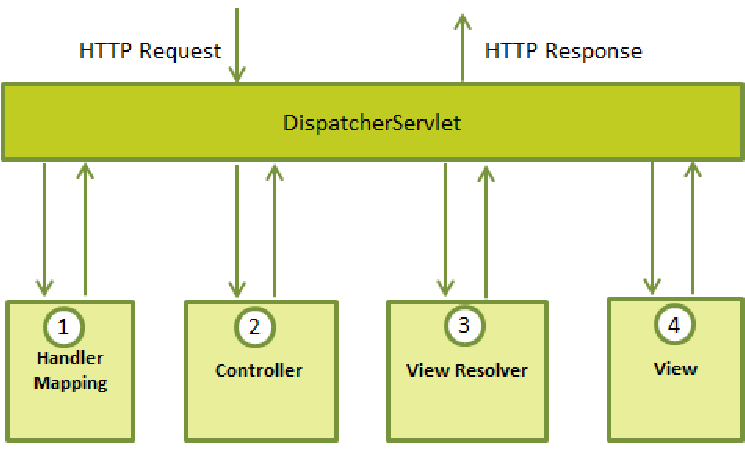
\includegraphics[scale=0.41]{img/obr3}
\end{center}
\begin{tikzpicture}[remember picture,overlay]
    \node[xshift=-0.6cm,yshift=-1.3cm] at (current page.north east){%
    
\includegraphics[width=1cm]{img/pozor}};
\end{tikzpicture} 
\end{frame}


\begin{frame}[fragile]\frametitle{Dispatcher servlet}
  \putat{-30}{-120}{
      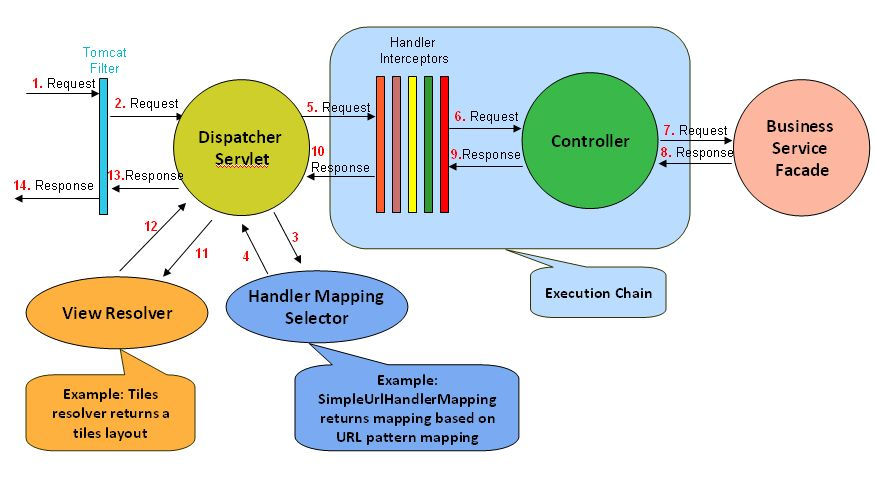
\includegraphics[width=12.7cm]{img/obr4}
    }
\end{frame}


\begin{frame}\frametitle{Dispatcher servlet}
	\begin{itemize}
		\item After receiving an HTTP request, \texttt{DispatcherServlet} consults the \texttt{HandlerMapping} to call the appropriate Controller.
        \medskip
		\item The Controller takes the request and calls the appropriate service methods based on used GET or POST method. The service method will set model data based on defined business logic and returns view name to the \texttt{DispatcherServlet}.
        \medskip
		\item The \texttt{DispatcherServlet} will take help from \texttt{ViewResolver} to pick up the defined view for the request.
        \medskip
		\item Once view is finalized, the \texttt{DispatcherServlet} passes the model data to the view which is finally rendered on the browser.
	\end{itemize}
\begin{tikzpicture}[remember picture,overlay]
    \node[xshift=-0.6cm,yshift=-1.3cm] at (current page.north east){%
    
\includegraphics[width=1cm]{img/pozor}};
\end{tikzpicture} 
\end{frame}


\begin{frame}[fragile]\frametitle{Configuration}
	\begin{itemize}
		\item Declare servlet in \texttt{web.xml}.
		\item Customize it in \verb+<appName>-servlet.xml+.
		\item Specify URL pattern to be handled (\texttt{*.jsp}).
		\item Enable Spring MVC annotation scanning.
          \begin{itemize}
        	\item \verb'<context:component-scan...>' 
          \end{itemize}
		\item Define controller and mapping.
	\end{itemize}
\end{frame}


\begin{frame}[fragile]\frametitle{Defining controller}
	\begin{itemize}
		\item The \texttt{@Controller} annotation defines the class as a Spring MVC controller.
        \medskip
		\item \texttt{@RequestMapping} annotation is used to map a URL to either an entire class or a particular handler method.
        \medskip
		\item Due to return value, redirection to \texttt{hello.jsp} will happen.
		\item[]
        	\medskip
			\begin{Verbatim}[fontsize=\footnotesize, commandchars=\\\{\}] 
@Controller
\textcolor{purple}{\textbf{public class}} HelloController \{
  @RequestMapping(value = \textcolor{blue}{"/hello"}, method = RequestMethod.GET)
  \textcolor{purple}{\textbf{public String}} printHello(ModelMap model) \{
    model.addAttribute(\textcolor{blue}{"message"},
      \textcolor{blue}{"Hello Spring MVC Framework!"});
    \textcolor{purple}{\textbf{return}} \textcolor{blue}{"hello"};
  \}
\}
			\end{Verbatim}
    \end{itemize}
\end{frame}


\begin{frame}[fragile]\frametitle{Creating JSP views}
	\begin{itemize}
		\item Here \texttt{\$\{message\}} is the attribute which we have setup inside the Controller. You can have multiple attributes to be displayed inside your view.
        \medskip
		\item File path will be \texttt{/WEB-INF/hello/hello.jsp}
		\item[]
        	\medskip
            \begin{verbatim}
<html>
    <head>
        <title>Hello Spring MVC</title>
    </head>
    <body>
        <h2>${message}</h2>
    </body>
</html>
            \end{verbatim}
	\end{itemize}
\begin{textblock}{15}(8.4,1.8)
    {\footnotesize Examples HelloWeb, SpringMVC}
\end{textblock}
\begin{tikzpicture}[remember picture,overlay]
    \node[xshift=-0.6cm,yshift=-1.3cm] at (current page.north east){%
    
\includegraphics[width=1cm]{img/naradi}};
\end{tikzpicture} 
\end{frame}



\begin{frame}\frametitle{Spring Security}
	\begin{itemize}
		\item Some pages should not be publicly available.
		\item Managing user roles
          \begin{itemize}
        	\item Users can view pages according to their user role level (user,~admin, super-admin).
          \end{itemize}
		\item Login
          \begin{itemize}
        	\item Default
              \begin{itemize}
            	\item Custom appearance may be defined.
              \end{itemize}
            \item HTTP
              \begin{itemize}
                \item HTTP Authentication (RFC 7235, 7615, 7616, 7617).
            	\item User logged in as long as browser runs.
              \end{itemize}
          \end{itemize}
	\end{itemize}
\begin{tikzpicture}[remember picture,overlay]
    \node[xshift=-0.6cm,yshift=-1.3cm] at (current page.north east){%
    
\includegraphics[width=1cm]{img/pozor}};
\end{tikzpicture} 
\end{frame}



\begin{frame}\frametitle{Spring security configuration}
	\begin{itemize}
		\item XML based
        \begin{itemize}
        	\item \texttt{web.xml}
        	\item \texttt{mvc-dispatcher-servlet.xml}
        	\item \texttt{spring-security.xml}
        \end{itemize}
		\item Annotation based
        \begin{itemize}
       	 	\item \texttt{@Configuration}
       	 	\item \texttt{@EnableWebSecurity}
       	 	\item \texttt{@EnableWebMVC} {\footnotesize -- imports the Spring MVC configuration}
       	 	\item \texttt{@ComponentScan}
        \end{itemize}
	\end{itemize}
\begin{tikzpicture}[remember picture,overlay]
    \node[xshift=-0.6cm,yshift=-1.3cm] at (current page.north east){%
    
\includegraphics[width=1cm]{img/oko}};
\end{tikzpicture} 
\end{frame}


\begin{frame}[fragile]\frametitle{XML configuration}
	\begin{itemize}
		\item \texttt{spring-security.xml}
        \item[]
        	\medskip
            \begin{Verbatim}[fontsize=\footnotesize, commandchars=\\\{\}]
\textcolor{red}{\textbf{<http}} \textcolor{purple}{\textbf{auto-config}}=\textcolor{blue}{"true"}\textcolor{red}{\textbf{>}}
  \textcolor{red}{\textbf{<intercept-url}} \textcolor{purple}{\textbf{pattern}}=\textcolor{blue}{"/admin**"} \textcolor{purple}{\textbf{access}}=\textcolor{blue}{"ROLE_USER"} \textcolor{red}{\textbf{/>}}

  \textcolor{red}{\textbf{<form-login}} 
    \textcolor{purple}{\textbf{login-page}}=\textcolor{blue}{"/login"}
    \textcolor{purple}{\textbf{default-target-url}}=\textcolor{blue}{"/welcome"} 
    \textcolor{purple}{\textbf{authentication-failure-url}}=\textcolor{blue}{"/login?error"} 
    \textcolor{purple}{\textbf{username-parameter}}=\textcolor{blue}{"username"}
    \textcolor{purple}{\textbf{password-parameter}}=\textcolor{blue}{"password"} \textcolor{red}{\textbf{/>}}
  \textcolor{red}{\textbf{<logout}} \textcolor{purple}{\textbf{logout-success-url}}=\textcolor{blue}{"/login?logout"}  \textcolor{red}{\textbf{/>}}
  \textcolor{olive}{\textbf{<!-- enable csrf protection -->}}
  \textcolor{red}{\textbf{<csrf/>}}
\textcolor{red}{\textbf{</http>}}

\textcolor{red}{\textbf{<authentication-manager>}}
  \textcolor{red}{\textbf{<authentication-provider>}}
    \textcolor{red}{\textbf{<user-service>}}
      \textcolor{red}{\textbf{<user}} \textcolor{purple}{\textbf{name}}=\textcolor{blue}{"user"} \textcolor{purple}{\textbf{password}}=\textcolor{blue}{"123456"}
            \textcolor{purple}{\textbf{authorities}}=\textcolor{blue}{"ROLE_USER"} \textcolor{red}{\textbf{/>}}
    \textcolor{red}{\textbf{</user-service>}}
  \textcolor{red}{\textbf{</authentication-provider>}}
\textcolor{red}{\textbf{</authentication-manager>}}
            \end{Verbatim}
	\end{itemize}
\begin{textblock}{15}(8.6,0.1)
    {\footnotesize Example SpringCustomSecurity}
\end{textblock}
\begin{tikzpicture}[remember picture,overlay]
    \node[xshift=-0.6cm,yshift=-1.3cm] at (current page.north east){%
    
\includegraphics[width=1cm]{img/oko}};
\end{tikzpicture} 
\end{frame}

\begin{frame}[fragile]\frametitle{XML configuration from 5.0.0.RC1}
	\begin{itemize}
		\item From version 5.0.0.RC1 \texttt{password-encoder} must be set.
        \item[]
        	\medskip
            \begin{Verbatim}[fontsize=\footnotesize, commandchars=\\\{\}]
\textcolor{red}{\textbf{<authentication-manager>}}
  \textcolor{red}{\textbf{<authentication-provider>}}
    \textcolor{red}{\textbf{<password-encoder}} \textcolor{purple}{\textbf{ref}}=\textcolor{blue}{"passwordEncoder"} \textcolor{red}{\textbf{/>}}
    \textcolor{red}{\textbf{<user-service>}}
      \textcolor{red}{\textbf{<user}} \textcolor{purple}{\textbf{name}}=\textcolor{blue}{"user"} \textcolor{purple}{\textbf{password}}=\textcolor{blue}{"123456"}
            \textcolor{purple}{\textbf{authorities}}=\textcolor{blue}{"ROLE_USER"} \textcolor{red}{\textbf{/>}}
    \textcolor{red}{\textbf{</user-service>}}
  \textcolor{red}{\textbf{</authentication-provider>}}
\textcolor{red}{\textbf{</authentication-manager>}}

\textcolor{red}{\textbf{<b:bean}} \textcolor{purple}{\textbf{id}}=\textcolor{blue}{"textEncryptor"} 
  \textcolor{purple}{\textbf{class}}=\textcolor{blue}{"org.springframework.security.crypto.encrypt.Encryptors"}
  \textcolor{purple}{\textbf{factory-method}}=\textcolor{blue}{"noOpText"} \textcolor{red}{\textbf{/>}}
		
\textcolor{red}{\textbf{<b:bean}} \textcolor{purple}{\textbf{id}}=\textcolor{blue}{"passwordEncoder"} 
  \textcolor{purple}{\textbf{class}}=
\textcolor{blue}{"org.springframework.security.crypto.password.NoOpPasswordEncoder"}
  \textcolor{purple}{\textbf{factory-method}}=\textcolor{blue}{"getInstance"} \textcolor{red}{\textbf{/>}}
            \end{Verbatim}
	\end{itemize}
\begin{textblock}{15}(8.5,1.1)
    {\footnotesize Example SpringCustomSecurity5}
\end{textblock}
\begin{tikzpicture}[remember picture,overlay]
    \node[xshift=-0.6cm,yshift=-1.3cm] at (current page.north east){%
    
\includegraphics[width=1cm]{img/oko}};
\end{tikzpicture} 
\end{frame}


\begin{frame}[fragile]\frametitle{Annotation configuration}
	\begin{Verbatim}[fontsize=\scriptsize, commandchars=\\\{\}]
@Configuration
@EnableWebSecurity
\textcolor{purple}{\textbf{public class}} AppSecurityConfig \textcolor{purple}{\textbf{extends}} WebSecurityConfigurerAdapter \{

  @Autowired
  \textcolor{purple}{\textbf{public void}} configureGlobal(AuthenticationManagerBuilder auth)
      \textcolor{purple}{\textbf{throws}} Exception \{
    auth.inMemoryAuthentication().withUser(\textcolor{blue}{"tom"}).
      password(\textcolor{blue}{"123456"}).roles(\textcolor{blue}{"USER"});
    auth.inMemoryAuthentication().withUser(\textcolor{blue}{"bill"}).
      password(\textcolor{blue}{"123456"}).roles(\textcolor{blue}{"ADMIN"});
    auth.inMemoryAuthentication().withUser(\textcolor{blue}{"james"}).
      password(\textcolor{blue}{"123456"}).roles(\textcolor{blue}{"SUPERADMIN"});
  \}

  @Override
  \textcolor{purple}{\textbf{protected void}} configure(HttpSecurity http) \textcolor{purple}{\textbf{throws}} Exception \{

    http.authorizeRequests()
      .antMatchers(\textcolor{blue}{"/protected/**"}).access(\textcolor{blue}{"hasRole('ROLE_ADMIN')"})
      .antMatchers(\textcolor{blue}{"/confidential/**"}).access(\textcolor{blue}{"hasRole('ROLE_SUPERADMIN')"})
      .and().formLogin();

  \}
\}
	\end{Verbatim}
\begin{textblock}{15}(7.8,0.5)
    {\footnotesize Example SpringSecurityAnnotations}
\end{textblock}
\end{frame}


\begin{frame}[fragile]\frametitle{Annotation configuration from 5.0.0.RC1}
	\begin{Verbatim}[fontsize=\scriptsize, commandchars=\\\{\}]
    auth.inMemoryAuthentication().withUser(\textcolor{blue}{"tom"}).
      password(\textcolor{blue}{"\{noop\}123456"}).roles(\textcolor{blue}{"USER"});
	\end{Verbatim}
\begin{textblock}{15}(7.7,6.9)
    {\footnotesize Example SpringSecurityAnnotations5}
\end{textblock}
\end{frame}


\begin{frame}[fragile]\frametitle{Password hashing}
	\begin{itemize}
		\item Supported password formats
        \begin{itemize}
        	\item \texttt{plaintext}
        	\item \texttt{sha}, \texttt{sha256}
        	\item \texttt{md4}, \texttt{md5}
            \item Integration with LDAP is possible.
            \item Newer versions supports also PBKDF2 (Password-Based Key Derivation Function 2), BCrypt, sCrypt, Argon2, \ldots
        \end{itemize}
        \item[]
        	\bigskip
  			\begin{Verbatim}[fontsize=\footnotesize, commandchars=\\\{\}]  
\textcolor{red}{\textbf{<authentication-manager>}}
  \textcolor{red}{\textbf{<authentication-provider>}}
    \textcolor{red}{\textbf{<password-encoder}} \textcolor{purple}{\textbf{hash}}=\textcolor{blue}{"sha"} \textcolor{red}{\textbf{/>}}
    \textcolor{red}{\textbf{<user-service>}}
      \textcolor{red}{\textbf{<user}} \textcolor{purple}{\textbf{name}}=\textcolor{blue}{"user"} 
            \textcolor{purple}{\textbf{password}}=\textcolor{blue}{"7c4a8d09ca3762af61e59520943dc26494f8941b"}
            \textcolor{purple}{\textbf{authorities}}=\textcolor{blue}{"ROLE_USER"} \textcolor{red}{\textbf{/>}}
    \textcolor{red}{\textbf{</user-service>}}
  \textcolor{red}{\textbf{</authentication-provider>}}
\textcolor{red}{\textbf{</authentication-manager>}}
   			\end{Verbatim}
    \end{itemize}
\end{frame}


\begin{frame}[fragile]\frametitle{CSRF exploit}
	\begin{itemize}
		\item Cross-site request forgery
          \begin{itemize}
        	\item Spring has to know, that the origin of the request to the admin section is from the trusted source (the form comes from this application and not from an attacker who sends a~request for example from an advertisement).
        	\item Otherwise hackers would be able to do exploit when the admin is logged in.
          \end{itemize}
        \medskip
		\item Post CSRF token in request
        \item[]
        	\medskip
			\begin{Verbatim}[fontsize=\footnotesize, commandchars=\\\{\}]  
\textcolor{red}{\textbf{<form}} \textcolor{purple}{\textbf{action}}=\textcolor{blue}{"${logoutUrl}"} \textcolor{purple}{\textbf{method}}=\textcolor{blue}{"post"} \textcolor{purple}{\textbf{id}}=\textcolor{blue}{"logoutForm"}\textcolor{red}{\textbf{>}}
  \textcolor{red}{\textbf{<input}} \textcolor{purple}{\textbf{type}}=\textcolor{blue}{"hidden"} \textcolor{purple}{\textbf{name}}=\textcolor{blue}{"${_csrf.parameterName}"}
         \textcolor{purple}{\textbf{value}}=\textcolor{blue}{"${_csrf.token}"} \textcolor{red}{\textbf{/>}}
\textcolor{red}{\textbf{</form>}}
            \end{Verbatim}
        \medskip
		\item Enable CSRF protection in configuration
          \begin{itemize}
            \item \verb+<csrf/>+
          \end{itemize}
	\end{itemize}
\begin{tikzpicture}[remember picture,overlay]
    \node[xshift=-0.6cm,yshift=-1.3cm] at (current page.north east){%
    
\includegraphics[width=1cm]{img/lupa}};
\end{tikzpicture}     
\end{frame}


\begin{frame}[fragile]\frametitle{Database login}
  \emph{Xml}
  \begin{Verbatim}[fontsize=\footnotesize, commandchars=\\\{\}]  
\textcolor{red}{\textbf{<authentication-manager>}}
  \textcolor{red}{\textbf{<authentication-provider>}}
    \textcolor{red}{\textbf{<jdbc-user-service}} \textcolor{purple}{\textbf{data-source-ref}}=\textcolor{blue}{"dataSource"} 
      \textcolor{purple}{\textbf{users-by-username-query}}=
        \textcolor{blue}{"select username,password,enabled from users where username=?"} 
      \textcolor{purple}{\textbf{authorities-}}\textcolor{purple}{\textbf{by-username-query}}=
        \textcolor{blue}{"select username,role from user_roles where username =?"}\textcolor{red}{\textbf{/>}}
 \textcolor{red}{\textbf{</authentication-provider>}}
\textcolor{red}{\textbf{</authentication-manager>}}

\textcolor{red}{\textbf{<bean}} \textcolor{purple}{\textbf{id}}=\textcolor{blue}{"dataSource"} \textcolor{purple}{\textbf{class}}=
    \textcolor{blue}{"org.springframework.jdbc.datasource.DriverManagerDataSource"}\textcolor{red}{\textbf{>}}
  \textcolor{red}{\textbf{<property}} \textcolor{purple}{\textbf{name}}=\textcolor{blue}{"driverClassName"} \textcolor{purple}{\textbf{value}}=\textcolor{blue}{"com.mysql.cj.jdbc.Driver"} \textcolor{red}{\textbf{/>}}
  \textcolor{red}{\textbf{<property}} \textcolor{purple}{\textbf{name}}=\textcolor{blue}{"url"} 
\textcolor{purple}{\textbf{value}}=\textcolor{blue}{"jdbc:mysql://localhost:3306/test?serverTimezone=Europe/Prague"} 
\textcolor{red}{\textbf{/>}}
  \textcolor{red}{\textbf{<property}} \textcolor{purple}{\textbf{name}}=\textcolor{blue}{"username"} \textcolor{purple}{\textbf{value}}=\textcolor{blue}{"springJDBC"} \textcolor{red}{\textbf{/>}}
  \textcolor{red}{\textbf{<property}} \textcolor{purple}{\textbf{name}}=\textcolor{blue}{"password"} \textcolor{purple}{\textbf{value}}=\textcolor{blue}{"password"} \textcolor{red}{\textbf{/>}}
\textcolor{red}{\textbf{</bean>}}
			\end{Verbatim}
\begin{tikzpicture}[remember picture,overlay]
    \node[xshift=-0.6cm,yshift=-1.3cm] at (current page.north east){%
    
\includegraphics[width=1cm]{img/oko}};
\end{tikzpicture} 
\end{frame}


\begin{frame}[fragile]\frametitle{Database login}
  \emph{Annotation}
  \begin{Verbatim}[fontsize=\footnotesize, commandchars=\\\{\}]  
@Autowired
DataSource dataSource;
@Autowired
\textcolor{purple}{\textbf{public void}} configAuthentication(AuthenticationManagerBuilder auth)
    \textcolor{purple}{\textbf{throws}} Exception \{
  auth.jdbcAuthentication().passwordEncoder(passwordEncoder())
    .dataSource(dataSource)
    .usersByUsernameQuery(
      \textcolor{blue}{"select username,password,enabled from users where username=?"})
    .authoritiesByUsernameQuery(
      \textcolor{blue}{"select username,role from user_roles where username=?"});
\}

@Bean
\textcolor{purple}{\textbf{public}} PasswordEncoder passwordEncoder() \{
  \textcolor{purple}{\textbf{return}} NoOpPasswordEncoder.getInstance();
\}
			\end{Verbatim}
\begin{textblock}{15}(8.5,1.6)
    {\footnotesize Example SpringDatabaseLogin}
\end{textblock}
\end{frame}

\begin{frame}\frametitle{Spring Boot}
  \begin{itemize}
    \item A preferred way how to create Spring applications
    \item Create stand-alone Spring apps
    \item Application server is embedded
    \item Opinionated starter dependencies
    \begin{itemize}
        \item \textit{"Convention over configurations"}
    \end{itemize}
    \item No XML configuration
    \item Provides a starter page for convenience
    \begin{itemize}
        \item \url{https://start.spring.io}
    \end{itemize}
  \end{itemize}
\end{frame}

\begin{frame}\frametitle{Spring Boot Apps - Typical Archictecture}
  \begin{itemize}
    \item Controllers
    \begin{itemize}
        \item Handle all HTTP related tasks
        \item Should contain no business logic
    \end{itemize}
    \item Services
    \begin{itemize}
        \item The business logic should be here
        \item Can contact other services or update the database via repositories
    \end{itemize}
    \item Repositories
    \begin{itemize}
        \item Essentially DAOs
        \item The code is mostly created automatically for us by Spring Data
    \end{itemize}
  \end{itemize}
\end{frame}



\begin{frame}\frametitle{References}
	\begin{itemize}
		\item Spring tutorial
          \begin{itemize}
        	\item \url{http://www.tutorialspoint.com/spring/index.htm}
          \end{itemize}
		\item Spring documentation
          \begin{itemize}
            \item \url{https://docs.spring.io/spring-framework/docs/}
        	\item \url{https://docs.spring.io/spring-framework/docs/5.3.x/}
        	\item \url{https://docs.spring.io/spring-framework/docs/5.2.9.RELEASE_to_5.2.10.RELEASE/}
          \end{itemize}
		\item Using Spring Handler Interceptors to Decouple Business Logic
          \begin{itemize}
        	\item {\footnotesize\url{https://sdevarapalli.wordpress.com/2011/02/16/using-spring-handler-interceptors-to-decouple-business-logic/}}
          \end{itemize}
		\item Overview of Spring MVC Architecture
          \begin{itemize}
        	\item \url{http://terasolunaorg.github.io/guideline/1.0.1.RELEASE/en/Overview/SpringMVCOverview.html}
          \end{itemize}
        \item Spring MVC Framework
          \begin{itemize}
        	\item \url{http://www.wideskills.com/spring/spring-mvc-framework}
          \end{itemize}
	\end{itemize}
\end{frame}

\begin{frame}\frametitle{References}
	\begin{itemize}
	    \item AOP
          \begin{itemize}
            \item \url{http://www.mkyong.com/spring/spring-aop-example-pointcut-advisor/}
            \item \url{http://www.byteslounge.com/tutorials/spring-aop-pointcut-advice-example}
          \end{itemize}
		\item Logout in Spring Security 4
          \begin{itemize}
        	\item \url{http://websystique.com/spring-security/spring-security-4-logout-example/}
          \end{itemize}
        \item Others
          \begin{itemize}
              \item \url{https://stackoverflow.com/questions/26515700/mysql-jdbc-driver-5-1-33-time-zone-issue}
              \item \url{https://github.com/spring-projects/spring-framework/wiki/Upgrading-to-Spring-Framework-5.x\#data-access-and-transactions}
              \item \url{https://www.baeldung.com/java-varargs}
              \item \url{https://stackoverflow.com/questions/53358568/springs-annotation-type-required-deprecation}
              \item \url{https://odrotbohm.de/2013/11/why-field-injection-is-evil/}
          \end{itemize}
	\end{itemize}
\end{frame}

\bluepage{Thank you for your attention!}



\end{document}
